\chapter{Fundamentação Teórica}
\label{chap:fundteorica}
Nessa parte será apresentados conceitos para melhor entendimento deste trabalho e da modelação utilizada. 
A seção \ref{chap:grafos} elucida o que são grafos e o capítulo \ref{chap:redecomplexa} explica a variação de grafo utilizado para modelar o problema proposto. Depois, na seção \ref{chap:lol} é esclarecido o ambiente que será abstraído, explicando algumas regras básicas do jogo.
\section{Grafos}
\label{chap:grafos}

Quando descrevemos uma situação utilizando pontos e ligações entre algum desses pontos, como o exemplo os pontos sendo pessoas, e as ligações entre as pessoas sendo as amizades feitas, a abstração matemática desse tipo dá lugar ao conceito de grafo \cite{Lucchesi1979}.

Segundo \citet{Viana2007} "Um grafo \(G(V, E)\) pode ser definido como um conjunto de vértices \(V\), e um conjunto de conexões \(E\) " e ele continua: "Cada elemento do conjunto \(E\), associa dois elementos do conjunto \(V\), assim, se \((u,v) \in E\), então existe uma conexão entre os vértices u e o vértice v ."

Os grafos também podem ser classificados como binários e não-binários, sendo os binários suas arestas representadas por 1 ( se existem ) ou 0 ( se não existem ), e os não-binários quando existe um conjunto W, onde informa a intensidade da interação de uma aresta entre dois vértices  \cite{Viana2007}.
(continua...)    

\section{Redes Complexas}
\label{chap:redecomplexa}
Sobre redes complexas, \citet{Viana2007} diz que é utilizado o termo redes complexas, quando um grafo representa um sistema físico real.  Então, levando em conta isso, um grafo do jogo LOL pode ser considerado como uma rede complexa.

(continua...)

Para que seja possível classificar os resultados adequadamente, serão apresentados três modelos que se destacam no estado da arte, as redes \textit{small worlds}, as redes livres de escala \citep{Albert2002}, e as redes aleatórias. E também será explicado sobre o coeficiente de aglomeração .

\subsection{\textit{Redes Small Worlds}}
 As redes \textit{small worlds}, são redes que, o caminho entre dois nós são relativamente pequenos. (continua...).
 
 
 \subsection{Redes Livres de Escala}
 Nas redes livres de escala, um nó tem a probabilidade \(P(k)\) de possuir \(k\) arestas obedecendo a lei da potência \(P(k) \sim k^{-y}\) \cite{Albert2002}, \cite{Antiqueira2005}. Segundo Matheus Palhares Viana, nas redes livres de escala, muitos nós tem poucas arestas, e poucos nós se ligam a muitos.
 
     
\subsection{Redes Aleatórias}
Segundo \citet{Viana2007}, as redes aleatórias são um sistema formado por E arestas e N vértices, onde as arestas são distribuídas aleatoriamente. \citet{CunhaRecuero2004} exemplifica esse tipo de rede como uma festa, “onde bastaria uma conexão entre cada um dos convidados, para que no fim dela, todos estejam conectados no fim dela” e que quanto mais conexões forem criadas, maior a chance de serem criados grupos de pessoas, e que de tempos se relacionarem com outros grupos, e que poderia concluir que esses nós se relacionarem de forma randômica.

 
 \subsection{Coeficiente de Aglomeração}
 Segundo \citet{Viana2007}, o coeficiente de aglomeração mede o quão conectado estão os nós da rede ou do grafo. \citet{Antiqueira2005}  define o coeficiente de aglomeração sendo:\[CA_i = \frac{E_i}{k_i(k_i-1)}\]


    \citet{Antiqueira2005}  continua: “Sendo para cada vértice \(i\) existe \(k_i\) arestas, que os ligam a outros \(k_i\) vértices. Se esses \(k_i\) vértices estivessem ligados diretamente à todos os outros vértices do conjunto, haveriam \(k_i(k_i- 1)\) arestas entre eles. E assumindo \(E_i\) o número de arestas que existentes entre os \(k_i\) vértices.	O coeficiente da rede inteira é a média de todos \(CA_i\)”


\

\begin{figure}[!ht]
	\caption{Coeficiente de aglomeração}
	\begin{center}
		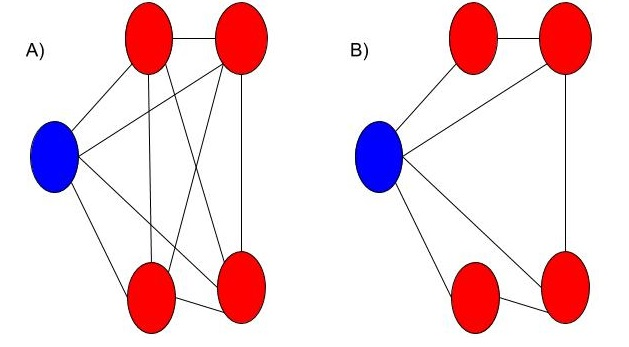
\includegraphics[width=15cm]{imagens/figura_grafos}
	\end{center}
	\small{Fonte: Autor (2018).}
	\label{fig:grafos}
\end{figure}

\
	No grafo A da Figura \ref{fig:grafos}, assumindo o peso de todas as arestas como 1, o coeficiente de aglomeração do vértice em azul é 1, e no grafo B o coeficiente do vértice em azul, segundo a fórmula é 12. 
    


\section{\textit{League of Legends}}
\label{chap:lol}
O jogo \textit{League of Legends}, é um jogo classificado como arena de batalha online de multi jogadores (do inglês \textit{Multiplayer Online Battle Arena} ) ou conhecido também como MOBA, que é um estilo de jogo onde, duas equipes se enfrentam em um campo de batalha, e cada jogador controla o seu personagem, mais chamado de herói ou campeão. O objetivo do MOBA é derrotar a equipe adversária destruindo a construção principal da equipe inimiga.

	A arena onde acontece o jogo é uma arena onde normalmente o mapa inicialmente é  espelhado,  ou  seja, o lado que cada time está,  não  oferece vantagens  exclusivas.  O mapa é composto  de  três caminhos até a base inimiga.
    
%%preciso conferir se essa foto é acervo, ou é do lol

\begin{figure}[!ht]
	\caption{Mapa do jogo de \textit{League of Legends}}
	\begin{center}
		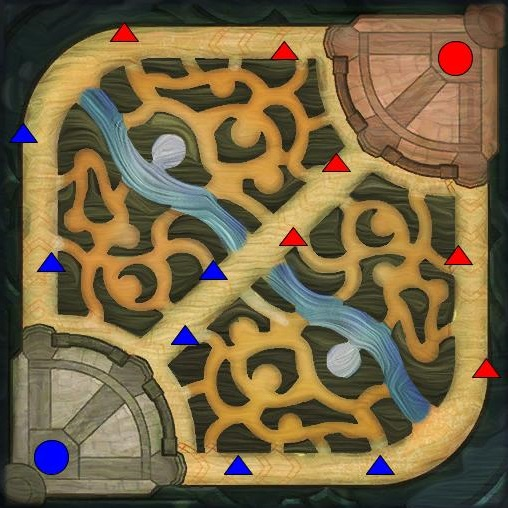
\includegraphics{imagens/mapa_lol.jpg}
	\end{center}
	\small{Fonte: Autor (2018).}
	\label{fig:mapa_lol}
\end{figure}

	A Figura \ref{fig:mapa_lol} mostra como é realmente o mapa do jogo, sendo que os círculos mostram a localização da construção principal, e os triângulos as construções de suporte de cada equipe, sendo azul uma equipe, e vermelho a outra.
    
	Com o início do jogo, cada jogador escolhe  um  herói  diferente, onde  cada  herói tem um conjunto de características únicas, como habilidades especiais,  seu impacto  no jogo  e  nas equipes adversárias e aliadas.
    
	Depois de escolher os heróis de cada equipe, cada jogador, deve procurar adquirir recursos no jogo, e objetivos para conseguir vantagens. Os recursos são limitados por equipe e por tempo, ou seja, deve ser bem escolhido quem ficará com a maior parte dos recursos da equipe.

\section{Estado da Arte}

No estado da arte, estudos com jogos de gênero MOBA são poucos, mas relacionados a redes complexas e predição existem diversos.

\subsection{Identifying Patterns in Combat that are Predictive of success}
 O trabalho de Yang \textit{et al}, relacionou a posição dos jogadores em uma batalha do MOBA com redes complexas, ao predizer o time vencedor daquela batalha.

\begin{figure}[!ht]
	\caption{As estruturas gráficas de uma batalha de MOBA}
	\begin{center}
		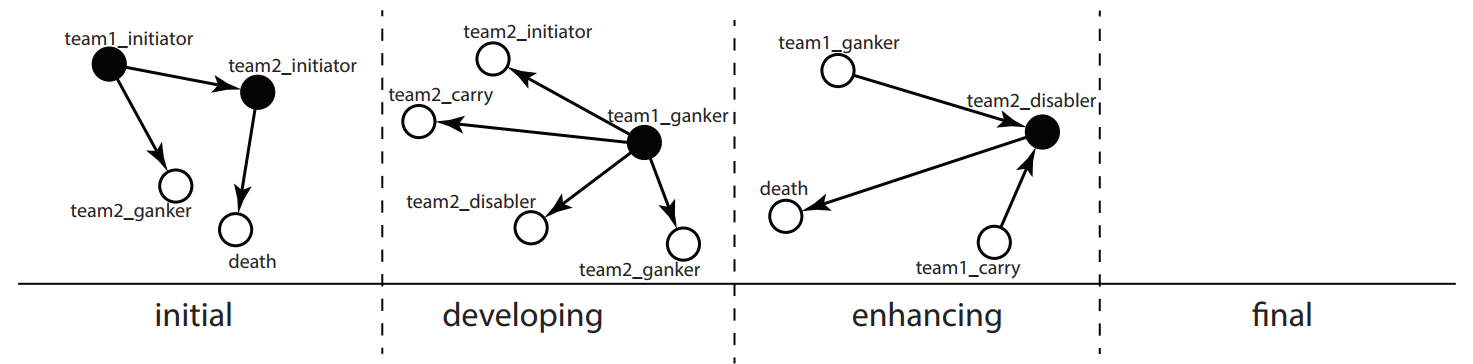
\includegraphics[width=15cm]{imagens/yang.PNG}
	\end{center}
	\small{Fonte: \cite{Yang2014}.}
	\label{fig:yang2014}
\end{figure}

Yang \textit{et al} modela os dados de um combate, em redes complexas, e treina uma arvore de decisão usando as melhores características tiradas dessa rede complexa. Depois de treinado a árvore, é identificado regras de combate que são preditivas de sucesso, e depois essas regras são traduzidas de volta em um padrão de combate específico usando uma técnica chamada mineração de subgrafo frequente.

\subsection{Análise de uma Métrica Alternativa para Predição de Laços Sociais em Grafos Lei de Potência}

Feito por \citeauthor{Danielewicz2016}, ela mostra uma visão geral do problema de predição de laços sociais, analisa os modelos de geração de grafos principalmente que seguem a lei da potência, no âmbito de formação de laços sociais e depois consegue uma métrica para predição de laços. Ela faz testes usando técnicas diferentes, mostrando seus resultados.